
\noindent \textbf{L3.4} No autômato generalizado da figura 1.67b, foi removido o estado 2, resultando no autômato da figura 1.67c. Foi então removido o estado 1 para produzir o autômato da figura 1.67d, obtendo-se assim uma expressão regular final. Refazer as contas produzindo um autômato generalizado ao se remover o estado 1 daquele da figura 1.67b. Deste autômato generalizado, remova o estado 2 e produza um novo autômato generalizado final com dois estados.

\textbf{Resposta:} 

\begin{center}
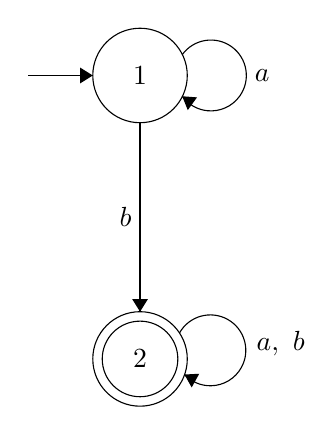
\begin{tikzpicture}[scale=0.2]
\tikzstyle{every node}+=[inner sep=0pt]
\draw [black] (7.9,-19.1) circle (3);
\draw (7.9,-19.1) node {$1$};
\draw [black] (7.9,-37.1) circle (3);
\draw (7.9,-37.1) node {$2$};
\draw [black] (7.9,-37.1) circle (2.4);
\draw [black] (0.8,-19.1) -- (4.9,-19.1);
\fill [black] (4.9,-19.1) -- (4.1,-18.6) -- (4.1,-19.6);
\draw [black] (7.9,-22.1) -- (7.9,-34.1);
\fill [black] (7.9,-34.1) -- (8.4,-33.3) -- (7.4,-33.3);
\draw (7.4,-28.1) node [left] {$b$};
\draw [black] (10.58,-17.777) arc (144:-144:2.25);
\draw (15.15,-19.1) node [right] {$a$};
\fill [black] (10.58,-20.42) -- (10.93,-21.3) -- (11.52,-20.49);
\draw [black] (10.399,-35.462) arc (150.971:-137.029:2.25);
\draw (15.27,-36.15) node [right] {$a,\mbox{ }b$};
\fill [black] (10.72,-38.09) -- (11.18,-38.91) -- (11.66,-38.04);
\end{tikzpicture}
\end{center}

\begin{center}
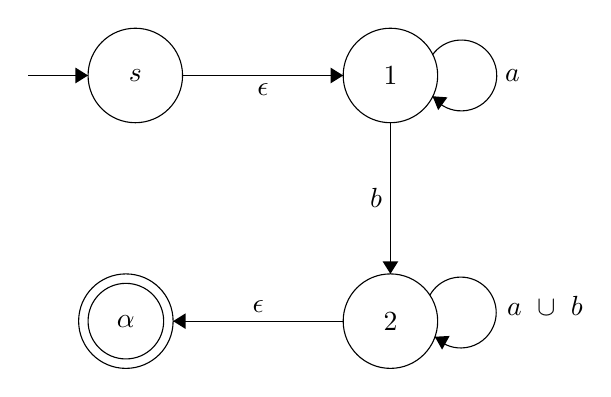
\begin{tikzpicture}[scale=0.2]
\tikzstyle{every node}+=[inner sep=0pt]
\draw [black] (39.5,-20.5) circle (3);
\draw (39.5,-20.5) node {$1$};
\draw [black] (39.5,-36.1) circle (3);
\draw (39.5,-36.1) node {$2$};
\draw [black] (23.3,-20.5) circle (3);
\draw (23.3,-20.5) node {$s$};
\draw [black] (22.7,-36.1) circle (3);
\draw (22.7,-36.1) node {$\alpha$};
\draw [black] (22.7,-36.1) circle (2.4);
\draw [black] (39.5,-23.5) -- (39.5,-33.1);
\fill [black] (39.5,-33.1) -- (40,-32.3) -- (39,-32.3);
\draw (39,-28.3) node [left] {$b$};
\draw [black] (42.18,-19.177) arc (144:-144:2.25);
\draw (46.75,-20.5) node [right] {$a$};
\fill [black] (42.18,-21.82) -- (42.53,-22.7) -- (43.12,-21.89);
\draw [black] (41.999,-34.462) arc (150.971:-137.029:2.25);
\draw (46.87,-35.15) node [right] {$a\mbox{ }\cup\mbox{ }b$};
\fill [black] (42.32,-37.09) -- (42.78,-37.91) -- (43.26,-37.04);
\draw [black] (16.5,-20.5) -- (20.3,-20.5);
\fill [black] (20.3,-20.5) -- (19.5,-20) -- (19.5,-21);
\draw [black] (26.3,-20.5) -- (36.5,-20.5);
\fill [black] (36.5,-20.5) -- (35.7,-20) -- (35.7,-21);
\draw (31.4,-21) node [below] {$\epsilon$};
\draw [black] (36.5,-36.1) -- (25.7,-36.1);
\fill [black] (25.7,-36.1) -- (26.5,-36.6) -- (26.5,-35.6);
\draw (31.1,-35.6) node [above] {$\epsilon$};
\end{tikzpicture}
\end{center}

Removendo o estado 1, onde $q_{rem} = 1, q_i = s, q_j = 2, R_1 = \epsilon, R_2 = a, R_3 = b, R4 = \emptyset$, temos $(\epsilon)(a)^*(b)\cup(\emptyset) = a^*b$:
\begin{center}
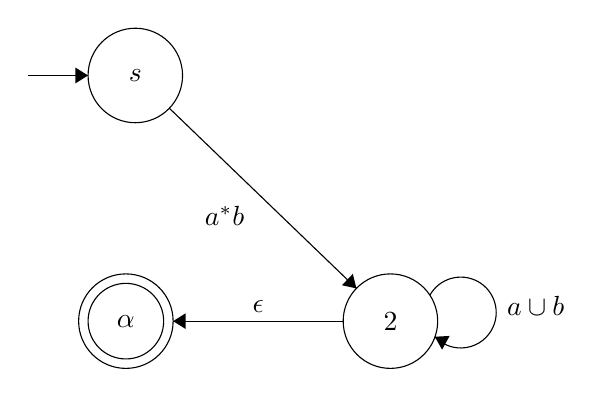
\begin{tikzpicture}[scale=0.2]
\tikzstyle{every node}+=[inner sep=0pt]
\draw [black] (39.5,-36.1) circle (3);
\draw (39.5,-36.1) node {$2$};
\draw [black] (23.3,-20.5) circle (3);
\draw (23.3,-20.5) node {$s$};
\draw [black] (22.7,-36.1) circle (3);
\draw (22.7,-36.1) node {$\alpha$};
\draw [black] (22.7,-36.1) circle (2.4);
\draw [black] (41.999,-34.462) arc (150.971:-137.029:2.25);
\draw (46.87,-35.15) node [right] {$a \cup b$};
\fill [black] (42.32,-37.09) -- (42.78,-37.91) -- (43.26,-37.04);
\draw [black] (16.5,-20.5) -- (20.3,-20.5);
\fill [black] (20.3,-20.5) -- (19.5,-20) -- (19.5,-21);
\draw [black] (36.5,-36.1) -- (25.7,-36.1);
\fill [black] (25.7,-36.1) -- (26.5,-36.6) -- (26.5,-35.6);
\draw (31.1,-35.6) node [above] {$\epsilon$};
\draw [black] (25.46,-22.58) -- (37.34,-34.02);
\fill [black] (37.34,-34.02) -- (37.11,-33.1) -- (36.42,-33.82);
\draw (28.97,-28.78) node [below] {$a^*b$};
\end{tikzpicture}
\end{center}

Removendo o estado 2, onde $q_{rem} = 2, q_i = s, q_j = \alpha, R_1 = a^*b, R_2 = a \cup b, R_3 = \epsilon, R4 = \emptyset$, temos $(a^*b) (a \cup b)^* (\epsilon)\cup(\emptyset) = (a^*b) (a \cup b)^*$:
\begin{center}
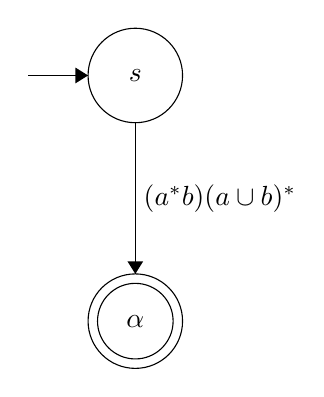
\begin{tikzpicture}[scale=0.2]
\tikzstyle{every node}+=[inner sep=0pt]
\draw [black] (23.3,-20.5) circle (3);
\draw (23.3,-20.5) node {$s$};
\draw [black] (23.3,-36.1) circle (3);
\draw (23.3,-36.1) node {$\alpha$};
\draw [black] (23.3,-36.1) circle (2.4);
\draw [black] (16.5,-20.5) -- (20.3,-20.5);
\fill [black] (20.3,-20.5) -- (19.5,-20) -- (19.5,-21);
\draw [black] (23.3,-23.5) -- (23.3,-33.1);
\fill [black] (23.3,-33.1) -- (23.8,-32.3) -- (22.8,-32.3);
\draw (23.8,-28.3) node [right] {$(a^*b)(a \cup b)^*$};
\end{tikzpicture}
\end{center}